\documentclass{article}
\usepackage[utf8]{inputenc}

\usepackage{graphicx}
\usepackage{float}
\usepackage{enumerate}
\usepackage{hyperref}
\hypersetup{
colorlinks=true,
linkcolor=blue,
filecolor=magenta, 
urlcolor=cyan,
}
\urlstyle{same}

\title{Project Imacs: System Requirements Specifications}
\author{Group 16:\\ Kelvin Lin\\ Jiahong Dong\\ Liam Casola\\ Varun Hooda\\ Mikolaj Hrycko\\ Danish Khan\\ Prince Sandu\\ Baltej Toor }
\date{November 2\textsuperscript{nd} 2018}

\begin{document}

\maketitle
\newpage
\tableofcontents
\newpage
\section{Introduction}
This section outlines the purpose and scope of Project Imacs, along with definitions, acronyms, and abbreviations used within this document. Its purpose is to set the context for the contents and organization of the software requirement document.

\subsection{Purpose}
This document's purpose is to outline the engineering and business requirements for Project Imacs. This document will be used to maintain a record of the project's scope, constraints, assumptions, dependencies, functional requirements, non-functional requirements, anticipated changes, and personas.

The target audience for this document are the stakeholders of this projects as well as any future software architects, designers, developers, and engineers.

\subsection{Scope}
This project will produce the following software products:

\begin{itemize}
\item A desktop client application.
\item A custom-made file system mapping a non-linear file structure to a linear one.
\end{itemize}

The aforementioned product will perform the following:

\begin{itemize}
\item Provide users with a graphical interface to organize files in a semantically consistent manner.
\item Provide users with a graphical interface to create and edit files.
\item Provide a means of persistent storage and retrieval of files.
\end{itemize}

The aforementioned product will not perform the following:

\begin{itemize}
\item Alter files outside the software ecosystem.
\item Persist files outside the user's local machine.
\item Infer relationships between files.
\item Automatically populate files with content.
\end{itemize}

\subsection{Definitions, Acronyms, and Abbreviations}
\subsubsection{File}
A file is a collection of data stored on the computer that can be interpreted into human-usable information by a computer. In this document, file is used interchangeably with notes; however, file is typically used to describe software behaviour while notes are typically used to describe user behaviour.

\subsubsection{Group of Files}
A group of files is a user-defined non-empty set of files that are related to each other. In this document, group of files is used interchangeably with group of notes; however, group of files is typically used to describe software behaviour while group of notes is typically used to describe user behaviour.

\subsubsection{Notes}
A note is a file with semantics; whereas a file can be a collection of arbitrary data, a note has meaning placed behind it by the user.

\subsubsection{Group of Notes}
A group of notes is a user-defined non-empty set of notes that are related to each other.

\subsubsection{Jump}
A jump is an operation that allows users to navigate the view between two related groups of files or two related groups of notes.

\subsubsection{Label}
A label is a unique user-defined textual description assigned to a group of files/notes to provide semantics for that group of files/notes.

\subsubsection{Relation}
A relation is a link between two different groups of files/notes.

\subsubsection{Software Ecosystem}
The software system is the collection of all files/notes that interact with Project Imacs. This includes any persistent data structures, any files that the user creates, and any files that the user imports into the software.

\subsubsection{Tag}
A tag is a user-defined textual description assigned to provide context to a file/note.

\subsection{References}
The following are references to existing note-taking and mind-mapping applications:

Microsoft OneNote: \url{https://products.office.com/en-CA/onenote}

GNU Emacs: \url{https://www.gnu.org/software/emacs/}

Visual Understanding Environment: \url{http://vue.tufts.edu/}

\subsection{Overview}
The rest of this document contains detailed descriptions of the project's requirements: assumptions, functionality, functional requirements, and non-functional requirements.

The other sections are organized into logical subsections. Section 2 outlines the overall product description with its various subsections. Section 3 will list the requirements. The functional requirements are organized by business events and viewpoints. Non-functional requirements are organized into various subcategories.

\section{Overall Description}
\subsection{Product Perspective}
Our system is an independent cross-platform desktop note-taking system with the ability to manage files. It allows the user to take notes in a non-linear file traversal system along a hierarchical file system. Users will be able to view and modify their files as well as the relation between files. Besides for the desktop operating system, such as but not limited to Windows and MacOS, the note-taking and file management system will not rely on any external software product. Nevertheless, in order to capture input from the user, the system requires either a keyboard, mouse, or touchpad. Users may choose to use a sketchpad or a digital pen instead of the aforementioned input systems and output devices. Some of the functionality in the system may require the use of external APIs; however, APIs will only act as add-on modules, and the core system that abstracts away hierarchical file management in the note-taking process will not be affected using APIs.

Similar systems to Project Imacs include Microsoft OneNote and Emacs. These solutions allow users to take and save notes; however, they fail to address the following problems:

\begin{itemize}
\item They do not allow the user to link physical files on their drive without duplicating the file or its contents resulting in lots of redundant information.
\item They do not allow for a distributed file handling format, resulting in large files that may be slow to load and corruption to the file may result in a lot of data loss.
\item The user can manually recreate a non-linear file system by creating separate folders; however, this will not allow them to visualize the relationship between the files.
\end{itemize}

Project Imacs will enable the user to group correlated notes in groups and non-hierarchically save them to the local machine.

\subsection{Product Functions}
In addition to the general note-taking functions that can be found in similar products, Project Imacs allows users to tag their notes, create relationship between correlated notes based on tags, and put these notes into groups. Users will be able to attach desired files to their notes. Users will also be able to save their notes in a non-hierarchical fashion on their local machines.

\subsection{User Characteristics}
Our note-taking system is intended for the general computer user with the desire to take notes and organize them in a non-linear manner. Potential users could be high school students, university students, working age adults, and mature adults.

\subsection{Constraints}
The system shall be constrained only by the user's operating system, and the physical computer hardware configurations.

\subsection{Assumptions and Dependencies}
It shall be assumed that the user does not violate any of the operating system's constraints. It shall also be assumed that the user is able and willing to use the appropriate hardware peripherals required to operate the system.
It shall be assumed that the user agrees to the terms and conditions of any licensing requirements specified by the APIs used in our application.

\section{Context Diagram}
The following context diagram illustrates the boundary of the Project Imacs system. The data element represents all utilized file system content and metadata. The Graphical User Interface component of Project Imacs provides the interface for the graphical manipulation of the data.

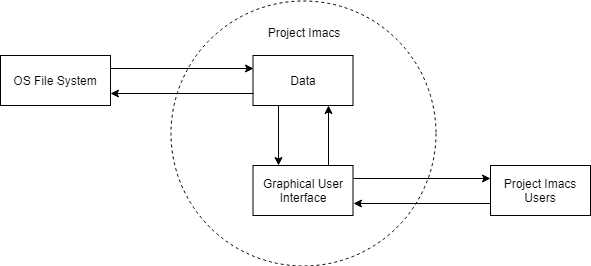
\includegraphics[scale=0.5]{context_diagram.png}

\section{Functional Decomposition Diagram}
The following is a functional decomposition diagram details top-level functional hierarchy of Project Imacs.

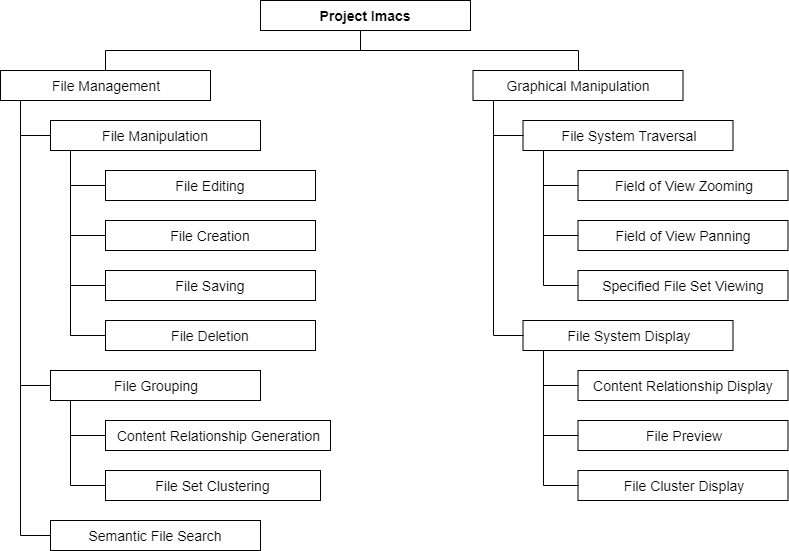
\includegraphics[scale=0.5]{functional_decomposition_diagram.png}

\newpage
\section{Functional Requirements}
\subsection{Data Requirements}
\begin{enumerate}[DR1]
\item The system shall allow the creation of files.

Rationale: The creation of files is needed in order to allow the user to create notes.
\item The system shall allow the addition of text, pen-input, or images to files.

Rationale: The addition of text, pen-input, and images is needed for the user to add content to their notes. Text, pen-input, and images were chosen as the required methods of input because it most closely relates to traditional note-taking using pen and paper. Relating Project Imacs to a familiar task will lower the cognitive effort required of the user to learn how to use the software.
\item The system shall allow the editing of files.

Rationale: The editing of files is needed to allow the user to correct mistakes they made while taking notes.
\item The system shall allow the deletion of content from files.

Rationale: The deletion of content from files is needed to allow users to remove incorrect, unwanted, or redundant information from their notes.
\item The system shall allow the saving of files.

Rationale: The saving of files is needed so that users will not have to re-enter their notes every time they use the software.
\item The system shall allow the retrieval of saved files.

Rationale: The user needs to be able to continue from a saved file or to read information from the saved file so that the information that the user previously entered is not lost.
\item The system shall allow for the incorporation external files into the software ecosystem.

Rationale: Some users may have used other note-taking/mind-mapping software before Project Imacs, and this requirement will facilitate their transition to Project Imacs resulting in a more intuitive user experience.
\item The system shall allow files to be assigned tags.

Rationale: Having a tag on files will allow users to provide context and descriptions for a file, and it will also facilitate the semantic search function defined in DR14, and the visualization requirement defined in UIR3.
\item The system shall allow files to be grouped together.

Rationale: Allowing files to be grouped together will allow the system to better visualize the relationship between files in requirement UIR2. It will also facilitate the semantic search function defined in requirement DR14.
\item The system shall allow a label to be assigned to a group.

Rationale: Allowing a label to be assigned to a group will enable the computer to visualize the label defined in UIR4, and it will aid in the semantic search function defined in requirement DR14.
\item The system shall allow relationships to be specified between groups of files.

Rationale: Allowing relationships to be specified between groups of files will allow the user to draw conclusions about how different notes relate to each other.
\item The system shall allow modification of the relationships between groups of files.

Rationale: Allowing the modification of relationships between groups of files is needed because the relationship between different group of files may change, and notes that were related in the past may not be related in the future.
\item The system shall allow jumping between related groups of files.

Rationale: Quick navigation between related groups of files is needed in order to facilitate an intuitive user experience.
\item The system shall allow searching for files semantically.

Rationale: Current note-taking and mind-mapping software does not allow users to search for content semantically; instead, they only allow users to search in-line text using exact word search or regular expression matching. Allowing users to search semantically will provide a better user experience that more naturally mimics human thought.
\item The system shall allow the deletion of files.
Rationale: The deletion of files is needed because the user will want to delete any notes that are no longer needed.
\end{enumerate}

\subsection{User Interface Requirements}
\begin{enumerate}[U{I}R1]
\item The system shall display the files stored within its ecosystem.

Rationale: The system needs to be able to display the files stored within its ecosystem because the user needs to be able to see their notes in order to read or make changes to them.
\item The system shall visualize the relationship between groups of files.

Rationale: The user needs to be able to see a visualization of the relationship between the groups of files because it will help them draw conclusions between how different sets of notes relate to each other.
\item The system shall display the tags associated with a file when the file is highlighted.

Rationale: Displaying tags is an important feature for enhancing usability because users can quickly see the context of the note and what the note is about.
\item The system shall display the label associated with a group of files when the group of files is presented on an output device.

Rationale: Displaying labels is an important feature because it allows users to see what each group of files represents, and this enhances the user experience.
\item The system shall show an interface for manipulating human-readable files.

Rationale: The user needs to be able to see the note in order to edit it.
\item The system shall allow navigation between relationships between groups of files.

Rationale: The user needs to be able to move between different files in order to modify different files.
\item The system shall allow users to change the notes visible on their screen.

Rationale: The user may want to focus on a particular note or decide to focus on a particular group of notes rather than the entire set of notes in the software ecosystem. In this case, the user must also be able to change the notes they see on the screen so that they are not permanently limited to seeing the notes that they decided to initially focus in on.
\item The system shall render images and plaintext files in a human usable format.

Rationale: Showing files in a human-readable format makes the user experience more intuitive because the user does not have to learn a new way of reading their notes.
\end{enumerate}

\newpage
\section{Non-Functional Requirements}
\subsection{Look and Feel Requirements}
\subsubsection{Appearance Requirements}
\begin{enumerate}[{A}PR1]
\item The application shall use appropriate font styling given the type and location of the text.

Rationale: Appropriate font styling and location of text is important to providing an intuitive user experience. If the font styling is inappropriate, the user may feel uncomfortable using it in professional environments. If the location of the text is inappropriate, the user may become frustrated trying to figure out where the different functions are located.
\item The application shall not have clashing colours that would make readability challenging for the user.

Rationale: Clashing colours could make it uncomfortable for some users to use the application, and users who feel strained by the colours may be discouraged from using the software.
\item The application shall visually resemble other business and note-taking applications.

Rationale: Having the application visually resemble other business and note-taking applications will allow the user to learn how to use the software faster. When users use the software, the bring with them past experience using other software. Their existing knowledge can be leveraged by using the same metaphors in the user interface for Project Imacs. This improves the user experience for the user.
\item The application shall prohibit users from interacting with the interactive elements that lead to invalid operations.

Rationale: When learning how to use our software, the user may inadvertently interact with interactive elements that could lead to data corruption or data loss if unguarded. This could lead to dissatisfaction or financial damage. Guarding users from performing invalid operations will protect the user against corrupting their own files.
\end{enumerate}

\subsubsection{Style Requirements}
\begin{enumerate}[STR1]
\item The visual style, colour palette, and fonts shall remain consistent throughout the application.

Rationale: Having consistent styling, colours, and fonts will improve the user experience because the user can learn to infer meaning, behaviour, and outcomes from interactive elements with certain colours.
\end{enumerate}

\subsection{Usability and Humanity Requirements}
\subsubsection{Ease of Use Requirements}
\begin{enumerate}[EUR1]
\item The application shall make the important features stand out.

Rationale: Having important features stand out improves user experience because it allows the user to find the most pertinent operations in the fastest time.
\item The application shall make the important features easily accessible.

Rationale: Having important features easily accessible is improves user experience because it allows the user to perform the most pertinent operations in the fastest time.
\end{enumerate}

\subsubsection{Learning Requirements}
\begin{enumerate}[LER1]
\item The product shall not require more than 20 minutes of training before the user can create notes, modify notes, group notes, and specify relationships between groups of notes.
Rationale: Users will become discouraged from using software if they cannot learn it within a reasonable amount of time. According to Wikipedia, the average sustained attention span of an adult is about 20 minutes (\url{https://en.wikipedia.org/wiki/Attention_span}). The key operations for Project Imacs are the ability to make notes, modify notes, group notes, and specify relationships between groups of notes. In order to maximize the user's comfort with the program, they should be able to learn how to use all the key operations of the application within one 20-minute sitting.
\end{enumerate}

\subsubsection{Understandability and Politeness Requirements}
\begin{enumerate}[UPR1]
\item The application shall have intuitive icons and appropriate names to describe the function of its interactive elements.

Rationale: Having intuitive icons and appropriate names to describe the function of the software's interactive elements allows the user to leverage past experiences to learn how to use Project Imacs faster.
\end{enumerate}

\subsubsection{Accessibility Requirements}
\begin{enumerate}[{A}CR1]
\item Text and graphic components shall be clearly distinguishable on the application interface.

Rationale: The user needs to be able to see the text and graphics in order to use the software.
\newpage
\item The application shall use a font size large enough to allow users to read the text.

Rationale: A small font size that is hard to read decreases usability because users will detract the user from the benefits of the program because they will spend time trying to read the text instead of taking notes. This may cause frustration and users may be discouraged from using the program.
\end{enumerate}

\subsection{Performance Requirements}
\subsubsection{Speed and Latency Requirements}
\begin{enumerate}[SLR1]
\item The system shall respond in real-time except in the cases of file searches and file operations.

Rationale: Current note-taking programs like OneNote operate in real-time and if the user experiences significant lag when typing or writing, then they will use another note-taking application instead.
\item The system shall perform search queries in less than 1 second per gigabyte of files in the software ecosystem.

Rationale: The user will not want to use software that take a long time to perform a search operation. A long delay may be perceived as faulty, and the user will stop using the software. 1 second per gigabyte was chosen because in an informal experiment performed by the group, it took on average 1 second to search for a file on the Windows operating system on a hard drive with 30GB of data. Given that semantic search is more complicated than inline text search, the rate of 1 second for 30GB of data was reduced to 1 second for 1GB of data.

\item The system shall open files and be ready for I/O operations in less than 2 seconds.

Rationale: Users would not want to wait for a long time before they are able to use the application. 2 seconds was chosen because, in an informal experiment performed by the group, it took on average 2 seconds to open Microsoft OneNote, another note-taking application.
\end{enumerate}

\subsubsection{Reliability and Availability Requirements}
\begin{enumerate}[R{A}R1]
\item The system shall have a 100\% uptime.

Rationale: Given that this application is a desktop application with no dependencies on external servers, the system should be up as long as the user's computer is operational.

\newpage
\item The system shall always make all data stored within its ecosystem available to the user through the application and through the user's operating system's default file management system.

Rationale: The requirement improves overall user experience because it allows the user to modify the files using more specialized software if they desire before returning to Project Imacs.
\end{enumerate}

\subsubsection{Robustness or Fault-Tolerance Requirements}
\begin{enumerate}[RFR1]
\item The system will keep data integrity upon spontaneous shutdown.

Rationale: The user should not lose data they previously saved if the system spontaneously shuts down, and the file contents should not be changed as to not confuse the user.
\item The system will automatically create backups of data.

Rationale: Automatically backing up the data will help ensure data integrity in the event of a system failure.
\end{enumerate}

\subsubsection{Capacity Requirements}
\begin{enumerate}[CR1]
\item The system must allow individual file sizes of up to 4GB.

Rationale: The maximum file amount of RAM supported by a 32-bit system is 4GB and allowing file sizes up to 4GB ensures cross-compatibility between 32-bit and 64-bit systems.
\item The system must allow total capacity file sizes of at least 128GB.

Rationale: Many laptops today have a minimum capacity of 128GB. This requirement ensures that the application will be supported on most modern-day laptops.
\end{enumerate}

\subsubsection{Scalability or Extensibility Requirements}
\begin{enumerate}[SER1]
\item The system shall be forwards compatible with new file formats.

Rationale: File formats and the kinds of data represented on computers change over time, and this requirement ensures that the software will be compatible with future file formats.
\item The system shall make its data available in a human-readable, non-proprietary format.

Rationale: This requirement improves user experience because it provides users with an audit trail of the software's operations.
\end{enumerate}

\subsubsection{Longevity Requirements}
\begin{enumerate}[LOR1]
\item The system shall use current software engineering standards and protocols.

Rationale: Using current standards and protocols allows for a mutual understanding between the engineers and developers of the software, and it allows the software to be maintained easier by future stakeholders.
\end{enumerate}

\subsubsection{Requirements for Interfacing with Adjacent Systems}
\begin{enumerate}[R{I}{A}1]
\item The application shall interface with all operating systems with a file system and a graphical user interface.

Rationale: The application should be platform-independent as long as the operating system provides the required components because different users may use different devices to access the application. This increases the overall reach of the software.
\item The application shall interface with the files provided by the user.

Rationale: Users may have existing notes on their computers that they want to import into Project Imacs' software ecosystem and enabling this lowers the barrier to entry for the user.
\end{enumerate}

\subsubsection{Productization Requirements}
\begin{enumerate}[PRO1]
\item The product shall be distributed as an executable file corresponding to the interfaced platform.

Rationale: The user needs to be able to run the software.
\end{enumerate}

\subsubsection{Release Requirements}
\begin{enumerate}[RR1]
\item New releases of the product shall be produced in conjunction with stakeholder and user feedback.

Rationale: In order to improve the product, stakeholders and users need to be consulted as they provide a different perspective of the software than the engineers.
\end{enumerate}

\subsection{Maintainability and Support Requirements}
\subsubsection{Maintenance Requirements}
\begin{enumerate}[MR1]
\item Maintenance of the software should not render the user's local copy unusable.

Rationale: As a standalone program, the user's software should not be affected by the maintenance of the code.
\end{enumerate}

\subsubsection{Supportability Requirements}
\begin{enumerate}[SUR1]
\item The software shall provide access to a help manual.

Rationale: Users may have questions about how to use certain features and functions of the software, and the help manual will provide users with that information.
\item A tutorial on the application's functionality shall be presented the first time the software is launched.

Rationale: The tutorial will help first-time users become proficient at the software quickly so that they can spend more time creating notes. This improves overall user experience.
\end{enumerate}

\subsection{Security Requirements}
\subsubsection{Access Requirements}
\begin{enumerate}[{A}CR1]
\item The system shall store associated files in a user-accessible location.

Rationale: The notes should not be hidden because users may decide to migrate from Project Imacs to another software application.
\end{enumerate}

\subsubsection{Integrity Requirements}
\begin{enumerate}[{I}NT1]
\item The system shall not introduce security vulnerabilities to the underlying OS file system structures.

Rationale: Users will not use a program if it compromises their computer system.
\item The system shall not create, corrupt, modify, or delete files not managed by the system.

Rationale: Users will not use a program if it could potentially damage the user's existing files.
\end{enumerate}

\subsubsection{Privacy Requirements}
\begin{enumerate}[PR{I}1]
\item The system shall not transmit or share the user's file contents and information.

Rationale: Users will not use a program if they found out that the software exposed their personal information to the public without their knowledge.
\item The system shall explicitly prompt the user to agree to any use of the user's data deviating from the core file management and manipulation functionality.

Rationale: Users will not use a program if they find out that it reads files that it is not supposed to without the user's consent.
\end{enumerate}

\section{Anticipated Changes}
\subsection{Likely Changes}
\subsubsection{Accessibility}
Accessibility requirements may change in the future to incorporate more accessible features so that the software can be used by a larger number of users. These changes may be brought about by changes in government regulations, demand from users, or demand from stakeholders. Such requirements may include:

\begin{itemize}
\item Restricting the colours used in the application to make the application more accessible to colour blind users.
\item Incorporating a high-contrast mode to make certain elements on the screen easier to see.
\item Incorporating text-to-speech to make the application more accessible to vision impaired and illiterate users.
\item Incorporating voice recording to make the application more accessible to vision impaired and illiterate users.
\item Incorporate screen reader functionality in the application to allow users to use a screen reader with the software.
\end{itemize}

\subsubsection{File Type Support}
Over time, different file types and forms of media are introduced, and users may have increased expectations for the kinds of media that the software system supports. Users may have changed expectations because the new file types make accomplishing a particular task easier or faster. Such can include:

\begin{itemize}
\item Support for music and sound files.
\item Support for embedded charts and spreadsheets.
\item Support for syntax highlighting for programming languages.
\item Support for 3D modelling files for augmented/virtual reality and 3D printing.
\item Support for running other executable files within Project Imacs.
\end{itemize}

\newpage
\subsubsection{Operating Platform}
Currently, the application runs locally on the user's computer. This requirement may change in the future as other operating platforms may allow for more people to use it at the same time, allow for larger files to be used, and provide an off-site backup of the user's data. The requirements may change in the future to allow:

\begin{itemize}
\item The software to run online.
\item The software to run in a distributed manner to support large files.
\item The software to run in a shared mode where multiple users can see the same notes.
\item The software to run in a shared mode where users can modify the notes and see other's changes in real time.
\end{itemize}

\subsubsection{Software Intelligence}
Expectations for software intelligence may increase in the future as developments in artificial intelligence and machine learning become more established. This could increase the number of features that users expect from a note taking application. Users may demand these additional features because it simplifies their workflow, and it makes them more productive. Additional requirements may include:

\begin{itemize}
\item Incorporating handwriting recognition to convert handwritten text into plaintext.
\item Incorporating handwriting recognition to convert handwritten mathematical equations into digital mathematical equations.
\item Automatically evaluating mathematical equations that the user enters the application.
\item Automatically linking keywords in a text document to internet articles that can provide more information.
\item Automatically identifying keywords and content in different files and automatically drawing links between different files.
\item Automatically summarizing the text in different files and answering user questions about the file.
\item Automatically checking spelling and grammar of different words.
\item Automatically predicting the user's next word as they type.
\item Automatically translating text in foreign languages.
\end{itemize}

\subsection{Unlikely Changes}
\subsubsection{Textual Notes}
It is unlikely that the requirement that system to support textual notes will change. This is because notes were traditionally taken as text, and it will take a long time to change the way society in general takes notes. Accordingly, even if there are newer, faster, or generally better ways of taking notes, it is unlikely that users will want to fully abandon textual note-taking as a possible alternative.

\subsubsection{Relating Files}
It is unlikely that the requirement that users can specify relationship between different files will change in the future. This is because the ability to relate files to each other form the basis for non-linear relationships. The ability to specify relationships between different files on the hard-drive ultimately forms the value proposition for Project Imacs.

\section{User Profiles and Personas}
\subsection{User Profiles}
Project Imacs' user interface will run on a user's laptop or desktop computer as an
native application. A set of attributes can be inferred about potential users based on
this previous assumption,

\begin{itemize}
\item Interested in something that just works with minimal overhead of setup and
learning
\item Reliability and availability held in high regard
\item Expect applications to be fast and not be a bottleneck when trying to carry out
a task
\item Application should work in a similar nature to other applications and
afford a similar set of capabilities
\end{itemize}

It is difficult to categorize users into a fix number of groups as each user's
expectations and exact requirements will be a bit different. But an overarching similarity
between users can be used to group users to broad groups,

\begin{itemize}
\item Students who take notes on computers
\item Professional who take notes on computers for work related tasks
\item Users who take personal notes for managing and organizing their lives, interests
and hobbies
\end{itemize}

\subsection{Personas}
A persona is a hypothetical individual that represents the typical user for Project Imacs. Based on independent research and speaking with people who currently use note taking software, we summarized some common personas for Project Imacs.

\subsubsection{Janet, Student}
Janet is a 20-year-old commerce student who is trying to understand how contribution margins effect a company's performance. She has notes on contribution margins; however, contribution margins affect many areas of businesses such as R\&D, marketing, operations, and finance. She wants to be able to relate contribution to each department's performance so that she can get a better sense of how the business performs overall.

\subsubsection{Timothy, Researcher}
Timothy is a 40-year-old researcher who classifies organisms for a living. He has notes for every organism he observes; however, he would like to be able to find organisms with similar attributes and group them together. Currently, he has a large database of animals, and he requires the help of an information technology student in order to effectively search and find the database. He would like to be able to visualize the different organisms he documented independently.

\end{document}

